\section{Power Dissipation in Resistors}

\instructornote{%
By Matt Trawick, 2015.  Time: $\sim$50 minutes

This is admitedly not the most sophisticated investigation we do, but several students have said this was their favorite lab all semester.

This lab assumes that students have already seen $P=IV$.  But for most students, just being introduced to it doesn't really teach them what power MEANS, in the very visceral sense of things becoming hot to the touch.

The write-up is deliberately somewhat minimalist.  You may need to tell students the ``Rated Power'' for the various resistors, as well as what that means (if you choose).  This lab also doesn't really explain what ``temperature coefficient'' means.   Students also may need some help using the resistor color code.

\textbf{Equipment notes: }

For the resistors, use 100 ohm resistors.  I've typically used:
\begin{itemize}[nosep]
\item 1/8 watt (Currently we have metal film resistors with a weakly positive temperature coefficient.)
\item 1/4 watt (I haven't used this lately.  Three resistors is really enough.)
\item 2 watt (Currently we have 2~W carbon-glass resistors with a strong negative temperature coefficient)
\item 25 watt (These are designed for high power, and should have a positive temperature coefficient, but one that's probably too small to measure.)  Incidentally, I think the 25~W rating is technically only for when its bolted to a heat sink, but they seem to do fine here.
\end{itemize}

The very smallest resistors can actually catch on fire, sometimes with a tiny burst of flame (smaller than a match) so be prepared.  The 2 W resistors will smoke and turn brown.  The biggest power resistors are totally unharmed.  
\textbf{By the way, it's always \textit{much} more memorable for the students if you don't tell them about the catching-on-fire part beforehand.  :-)}

For the multimeters, have some extra fuses on hand, as some fuses may be blown.  However, we can minimize this by presetting the current limiter knobs to just over 300 mA. (Setting the coarse adjustment knob fully counter-clockwise and the fine adjustment knob fully clockwise limits the supply to about what we need.)  Since we're using 100~$\Omega$ resistors, all currents should be safely below the 500~mA rating of the DMM fuses, so even without the current limit, we shouldn't blow any fuses unless students short their wires together.  Which some will.
}

\makelabheader %(Space for student name, etc., defined in master.tex)

\bigskip
\textbf{Apparatus}
\begin{itemize} [nosep]
\item digital multimeters (2)
\item DC power supply 
\item various resistors
\item banana cables and aligator clips
\end{itemize}

\textbf{Activity 1: Measuring Resistances}

(a) You have at your lab station several different resistors: some small ones with colored bands around them, and one much larger one encased in bronze-colored metal.  Write a brief description of each resistor along with their ``nominal'' resistances (that is, the values they're supposed to have) in the table below.  Some resistors have their nominal resistance $R$ printed directly on them.  For the smaller resistors with colored bands, you can find thier nominal resistance using the resistor color code as described in Appendix \ref{resistor_code}.  

\begin{center}
{\renewcommand{\arraystretch}{2.0}
\begin{tabular}{|C{3.8in}|c|c|c|} \hline 
Physical description, size, and colors of bands (if applicable) & Nominal $R$ & Measured $R$ & Rated Power \\ 
\hhline{|=|=|=|=|}
& & & \\ \hline 
& & & \\ \hline 
& & & \\ \hline 
& & & \\ \hline 
\end{tabular} }
\end{center}

(b) Measure the actual resistance of each resistor using your digital multimeter (DMM), and record your values in the table above.  To measure resistance, set the DMM to ``$\Omega$'' and put the two leads in the jacks labeled ``COM'' and ``V-$\Omega$''.  Are your measurements consistent with the nominal value of each resistor, to within their stated tolerances?
\answerspace{0.6in}

(c) What is the relationship between the physical size of the resistors and their resistance?
\answerspace{0.8in}

\begin{wrapfigure}[6]{r}{0.2\textwidth}
    \vspace{-0.5 in}
    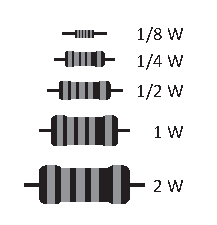
\includegraphics{electric_power/resistor_sizes.eps}
\end{wrapfigure}

(d) Write the ``rated power'' of each resistor in your table.  This is the maximum power a resistor can dissipate while still maintaining its characteristics.  Large resistors often have their rated power printed directly on them.  For the smaller ones, you would need to look at the label on the box they came in to know for sure, but you can generally estimate the rated power from the size of the resistor, based on the life-sized drawing to the right. 


\pagebreak
\textbf{Activity 2: Measuring Voltage, Current, and Power}

\begin{wrapfigure}[8]{r}{0.3\textwidth}
    \vspace{-0.4 in}
    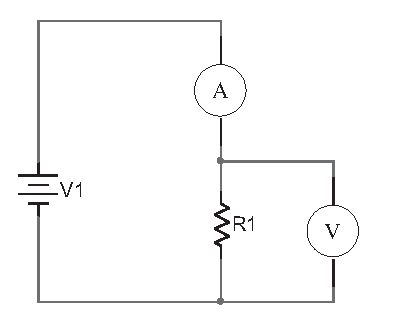
\includegraphics[width=0.3\textwidth]{electric_power/circ_diagram_bw.eps}
\end{wrapfigure}

(a) Connect the physically largest resistor to the power supply as shown in the circuit diagram to the right, using two multimeters to precisely measure both the current $I$ and the voltage drop $\Delta V$ across the resistor.  As you increase the voltage across the resistor, calculate both the power $P$ dissipated in it, and its resistance as calculated by $\Delta V/I$.  At each value, feel the resistor (\textit{carefully, so you don't burn your fingers!}) to see if it is getting hot.  To get accurate current readings, use the smallest current range you can.

\vspace{0.2in}

%\begin{center}
%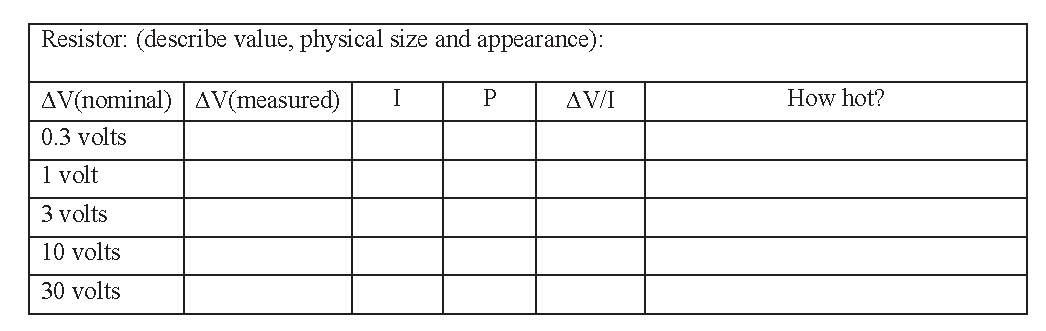
\includegraphics[width=1.0\textwidth]{electric_power/iv_table.eps}
%\end{center}

\newcommand{\maketableforivmeasurements}{
\begin{center}
{\renewcommand{\arraystretch}{2.0}
\begin{tabular}{|l|c|C{0.6in}|C{0.6in}|c|C{2.0in}|} \hline 
\multicolumn{6}{|l|}{Resistor (physical size, appearance, and value):} \\
\hline
$\Delta V$ (nominal) & $\Delta V$ (measured) & $I$ & $P$ & $\Delta V / I$ ($\Omega$) & How hot?\\ 
\hhline{|=|=|=|=|=|=|}
0.3 volts & & & & & \\ \hline 
1 volt & & & & & \\ \hline 
3 volts & & & & & \\ \hline 
10 volts & & & & & \\ \hline 
30 volts & & & & & \\ \hline 
\end{tabular} }
\end{center}
}
\maketableforivmeasurements

(b)  Based on your measurements, did the resistance increase, decrease, or stay the same as you increased the current?  (Be careful: are your measurements of current and voltage precise enough to support your conclusion?)  Is the temperature coefficient positive or negative for this resistor? 
\answerspace{1.0in}

\begin{center}
\framebox[1.07\width]{\textit{This is a good time to check with your instructor to be sure your measurements are on the right track.}} \par
\end{center}

(c) Now repeat your measurements for each of the other resistors, recording results in the tables below.  \textit{Again, be careful not to burn your fingers!}

\maketableforivmeasurements

\maketableforivmeasurements

\maketableforivmeasurements


(d) Now that they are no longer hot, make a final resistance measurement for each resistor (or whatever is left of it).  Have any of their resistances changed permanently?
\answerspace{1.0in}

(e) Can you determine the sign of the temperature coefficient (positive or negative) for any of your resistors?
\answerspace{1.0in}


(f) What difference did the physical size of the resistor make in the results of any of your measurements?  (Like, for instance, how hot they got and which resistors survived the experiment.)  Why did size make a difference?
\answerspace{1.0in}






